% !TeX root = ../main.tex
\chapter{Introduction and outline}
\label{chap:introduction}

\section{Quantum chromodynamics and its and phase diagram}
\begin{figure}[htp]
    \centering 
    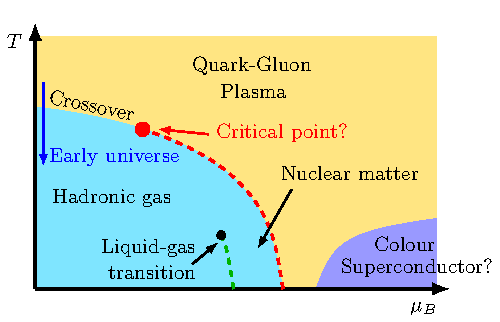
\includegraphics[scale=1.0]{figures/phase_diagram.pdf}
    \caption{}
    \label{fig:QCD_phase_diagram}
\end{figure}
The phase diagram of Quantum Chromodynamics (QCD) stands as a captivating yet challenging terrain, encapsulating the diverse phases of matter under varying conditions of temperature and baryon density. At the heart of this diagram lies the intricate interplay between hadronic matter, characterized by the confinement of quarks and gluons within protons and neutrons, and the elusive quark-gluon plasma, a state believed to have existed microseconds after the Big Bang. Bridging these extremes are regions of phase transitions and critical points, where subtle changes in the system lead to transformative alterations in its properties.
Investigating the QCD phase diagram is a formidable task, primarily due to the nonperturbative nature of the strong force. Analytical methods, often successful in perturbative regimes, falter in the face of the intense interactions among quarks and gluons at lower energy scales. This necessitates the use of numerical techniques, with lattice QCD simulations being a prominent approach. However, the lattice discretization introduces its own set of challenges, such as finite volume effects and the need for extrapolations to the continuum limit, adding layers of complexity to the study.
Moreover, the precise determination of the location and nature of the critical point remains an unresolved puzzle, requiring sophisticated tools and innovative methodologies. Theoretical predictions must be juxtaposed with experimental observations, further complicating the quest for a comprehensive understanding of the QCD phase diagram.
\section{The emergence of effective theories}
A central role in our investigation will be played by the Wilsonian perspective of the Renormalization Group (RG). Within this paradigm, renormalization ceases to be merely a tool for taming divergences; 
the Wilsonian RG approach provides a way to resolve physics at different scales. The Wilson framework naturally brings to the concept of effective theory, a model which describes phenomena only in terms of relevant degrees of freedom. In the context of QCD, a diverse array of effective theories are introduce, tailored to specific aspects of the strong force dynamics. 
Some examples are the Quark Meson Model provides a framework for studying the interplay between quarks and mesons, shedding light on the transition between confined and deconfined phases.
The Nambu-Jona-Lasinio model, explores the dynamical breaking of chiral symmetry and its consequences for hadron masses. This effective theory, rooted in the spontaneous symmetry breaking mechanism, offers valuable insights into the behavior of quarks and gluons in the low-energy regime.
Another notable effective theory, the Gross-Neveu model, delves into the dynamics of massless fermions and their interactions, exhibiting chiral symmetry breaking and providing a simplified yet insightful perspective on certain aspects of QCD.
The Gross-Neveu model, initially conceived in the realm of particle physics, finds surprising applications in condensed matter physics. Notably, it has been instrumental in the study of BCS superconductivity theory. The Gross-Neveu model's insights into the dynamics of massless fermions and its ability to describe chiral symmetry breaking have proven to be valuable in understanding the emergence of superconducting states in certain condensed matter systems. 
\section{Lattice Field Theory}
\vspace{20pt}
Computing physical quantities from first principle approaches, is not only hard to do, but results often impossible due to the appearence of divergences in the calculations. To fix this, one often relies on expansion techniques such as perturbation theory (\textcolor{red}{CITATION}), in which one tries to regularise the theory order by order in an expansion on the interaction coupling, yielding finite quantities that depend on the truncation order.  While this method is capable of producing incredibly precise results (\textcolor{red}{g-2, fine structure, ...}), it fails completely in treating non-perturbative phenomena, namely effects that cannot be captured by any order in the expansion or that are typical of strongly interacting systems. Example of such systems range from \textcolor{red}{QCD, cold atoms, plasma, stuff}. 
Moreover, such formulation is also not much suitable for numerical computations, since both the path integral and action measure are infinite dimensional objects. \\
Lattice field theory \cite{Montvay1994QuantumLattice,rothe_LGT,gattringer_LQCD,creutz_2023} is meant at first as a powerful non-perturbative regularisation tool to prevent divergences to occur and render the computation of the correlation functions finite. Moreover, it also provides a framework to study quantum field theory numerically on a computer. In order to accomplish this, one typically defines the theory on a spacetime lattice and makes use of statistical methods such as Monte Carlo algorithms to compute observables. One may wonder how can one reconstruct the results in the continuum theory, keeping the results finite, and matching the results on the discretised theory to physically measured ones. This task, far from beeing simple, will be the focus of the next sections, in which we will first introduce relevant theoretical tools, such as the renormalisation group, and then discuss the existence of a continuum limit of a lattice theory and, if it exists, how it can be extracted. This will motivate the introduction of coloured noise in the context of continuum limits of effective theories, a technique which will be shown to be powerful also for other various reasons, which will be the main focus of the analysis carried in the remaining chapters. \\
We want to mention that the Yukawa theory \eqref{eq:full_action_continuum} includes, as a special case, the Gross-Neveu model \textcolor{red}{citation}, which in turn is the 1+1 dimensional version of the Nambu-Jona-Lasinio model \cite{Nambu1961DynamicalI, Nambu1961DynamicalII}.
More precisely, after dynamical bosonisation via a Hubbard-Stratonovich transformation \textcolor{red}{either cite or show}, the latter theories reduce to a Yukawa model with 
\begin{equation*}
    K(x,y) = m_\phi^2 \, \delta(x,y) \qquad \lambda = 0.
\end{equation*}
\textcolor{red}{Da qualche parte cita \cite{carosso2020novel}}

\newpage 
\section{Outline}
Chapter \ref{chap:background} will be devoted to the introduction of the theoretical background that supports this work. 
We will start with the Kadanoff and Wilson approach to renormalisation in statistical physics and quantum field theory. 
Lattice field theory will then be introduced as a powerfool tool to simulate quantum field theory numerically and the basics of the formulation will be provided. 
We then turn to stochastic quantisation, the relation between noise and quantum fluctuations and how the standard formulation is modified by the presence of coloured noise. 
This will results in a deep connection between coloured stochastic quantisation and the renormalisation group.
The chapter will end with a description of the model on which the above techniques are applied, namely a Yukawa theory. \\~\\
Chapter \ref{chapt:methods} is devoted to detail techniques and methodologies of the project. We will start by explaining how the continuum model is discretised on a space-time lattice and how it can be simulated via a Monte Carlo method and stochastic quantisation. \\
We will then list some possible applications of coloured noise in lattice QFT and describe some of the numerical experiments that will be carried in the last chapter.\\
The chapter will end with a description of the relevant observables that are employed to study a lattice quantum field theory. \\~\\
Chapters \ref{chapt:results_preliminary} and \ref{chapt:results_coloured} are devoted to the numerical investigation. \\
First, some premilinary analysis will be carried. We will show how fermionic masses are measured in the simulation and provide a panoramic over the general phase structure of the theory. The latter will guide the choice of parameter settings for all the simulations. \\
It will then be showed how coloured noise can be used to provide a smooth interpolation between the fully classical and fully quantum picture. \\
The introduction of noise can cause qualitative change in the behaviour of the system. In particular, it will be shown how quantum fluctuations can trigger a chiral phase transition in the model. \\
Finally we will show how coloured noise in combinations with the Kadanoff-Wilson RG can be used to cool a simulation by systematically encoding UV fluctuations in a redefinition of the classical action, without altering the physical content of the theory.